\chapter{平方根アルゴリズム - Square root algorithms}

\index{square root algorithm}

A \key{平方根アルゴリズム(square root algorithm)} は、時間計算量が平方根になるアルゴリズムの相性です。
平方根は「貧乏人の対数(poor man's logarithm)」です。
$O(\sqrt n)$はO(n)より高速に動作しますが$O(log n)$よりは遅いです。
とはいえ、多くの平方根アルゴリズムは高速に動作し、競技プログラミングでは実際に使用することができます。

例を挙げて考えます。、配列に対して、あるindexの要素を変更する操作と、与えられた区間の合計を計算する操作の2つをサポートするデータ構造を考えます。
この問題は本書でもみてきた通り、バイナリインデックス木やセグメントツリーを用いることで$O(log n)$で両方の操作で解くことができます。
ここでは、$O(1)$時間で要素を修正し、$O(\sqrt n)$で合計を計算できる平方根アルゴリズムを使って、この問題にアプローチします。

これは、配列をサイズ $\sqrt n$の\emph{ブロック}に分割し、各ブロックにブロック内の要素の合計が含まれるようにします。
例えば、$n=16$要素の配列は、以下のように4要素のブロックに分割されます。

\begin{center}
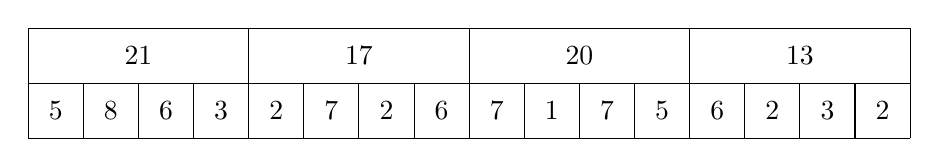
\begin{tikzpicture}[scale=0.7]
\draw (0,0) grid (16,1);

\draw (0,1) rectangle (4,2);
\draw (4,1) rectangle (8,2);
\draw (8,1) rectangle (12,2);
\draw (12,1) rectangle (16,2);

\node at (0.5, 0.5) {5};
\node at (1.5, 0.5) {8};
\node at (2.5, 0.5) {6};
\node at (3.5, 0.5) {3};
\node at (4.5, 0.5) {2};
\node at (5.5, 0.5) {7};
\node at (6.5, 0.5) {2};
\node at (7.5, 0.5) {6};
\node at (8.5, 0.5) {7};
\node at (9.5, 0.5) {1};
\node at (10.5, 0.5) {7};
\node at (11.5, 0.5) {5};
\node at (12.5, 0.5) {6};
\node at (13.5, 0.5) {2};
\node at (14.5, 0.5) {3};
\node at (15.5, 0.5) {2};

\node at (2, 1.5) {21};
\node at (6, 1.5) {17};
\node at (10, 1.5) {20};
\node at (14, 1.5) {13};

\end{tikzpicture}
\end{center}


配列要素の変更は、変更のたびに1ブロックの合計を更新すれば よいので$O(1)$で行えます。
次の図のように値自身とブロックの値を考えれば良いです。

\begin{center}
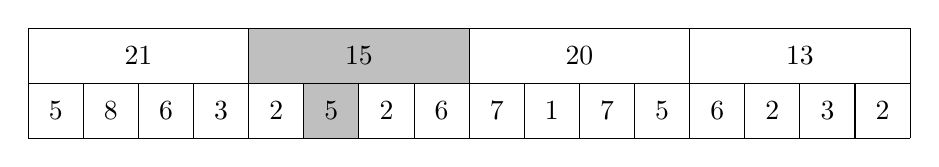
\begin{tikzpicture}[scale=0.7]
\fill[color=lightgray] (5,0) rectangle (6,1);
\draw (0,0) grid (16,1);

\fill[color=lightgray] (4,1) rectangle (8,2);
\draw (0,1) rectangle (4,2);
\draw (4,1) rectangle (8,2);
\draw (8,1) rectangle (12,2);
\draw (12,1) rectangle (16,2);

\node at (0.5, 0.5) {5};
\node at (1.5, 0.5) {8};
\node at (2.5, 0.5) {6};
\node at (3.5, 0.5) {3};
\node at (4.5, 0.5) {2};
\node at (5.5, 0.5) {5};
\node at (6.5, 0.5) {2};
\node at (7.5, 0.5) {6};
\node at (8.5, 0.5) {7};
\node at (9.5, 0.5) {1};
\node at (10.5, 0.5) {7};
\node at (11.5, 0.5) {5};
\node at (12.5, 0.5) {6};
\node at (13.5, 0.5) {2};
\node at (14.5, 0.5) {3};
\node at (15.5, 0.5) {2};

\node at (2, 1.5) {21};
\node at (6, 1.5) {15};
\node at (10, 1.5) {20};
\node at (14, 1.5) {13};

\end{tikzpicture}
\end{center}

さて、ある範囲の要素の総和を計算するために、範囲を3つに分割します。
両端にはみ出した要素が両端、と、その間のブロックの3つで、この総和を求めることにします。

\begin{center}
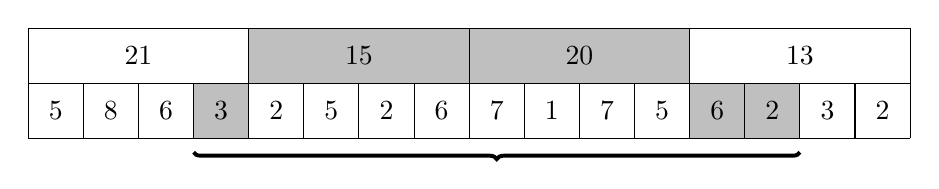
\begin{tikzpicture}[scale=0.7]
\fill[color=lightgray] (3,0) rectangle (4,1);
\fill[color=lightgray] (12,0) rectangle (13,1);
\fill[color=lightgray] (13,0) rectangle (14,1);
\draw (0,0) grid (16,1);

\fill[color=lightgray] (4,1) rectangle (8,2);
\fill[color=lightgray] (8,1) rectangle (12,2);
\draw (0,1) rectangle (4,2);
\draw (4,1) rectangle (8,2);
\draw (8,1) rectangle (12,2);
\draw (12,1) rectangle (16,2);

\node at (0.5, 0.5) {5};
\node at (1.5, 0.5) {8};
\node at (2.5, 0.5) {6};
\node at (3.5, 0.5) {3};
\node at (4.5, 0.5) {2};
\node at (5.5, 0.5) {5};
\node at (6.5, 0.5) {2};
\node at (7.5, 0.5) {6};
\node at (8.5, 0.5) {7};
\node at (9.5, 0.5) {1};
\node at (10.5, 0.5) {7};
\node at (11.5, 0.5) {5};
\node at (12.5, 0.5) {6};
\node at (13.5, 0.5) {2};
\node at (14.5, 0.5) {3};
\node at (15.5, 0.5) {2};

\node at (2, 1.5) {21};
\node at (6, 1.5) {15};
\node at (10, 1.5) {20};
\node at (14, 1.5) {13};

\draw [decoration={brace}, decorate, line width=0.5mm] (14,-0.25) -- (3,-0.25);

\end{tikzpicture}
\end{center}

単体の要素数は$O(\sqrt n)$、ブロック数も$O(\sqrt n)$であるからであるため、
和の問い合わせは$O(\sqrt n)$となります。
ブロックサイズ$O(\sqrt n)$とした目的は、配列が$O(\sqrt n)$個のブロックに分割されて、
各ブロックも$O(\sqrt n)$個の要素を含むという2つを達成することです。

尚$\sqrt n$の値は正確である必要はありません。
例えば、パラメータ$k$を用いて、$k$が$\sqrt n$と異なる$n/k$を用いてもよいです。
最適なパラメータは問題や入力に依存します。
例えば、ブロック全体は頻繁に参照されるが、ブロックの中の要素を見ることがほとんどないなら、
配列を$k < \sqrt n$ブロックに分割し、それぞれが、$n/k > \sqrt n$ の要素を含むようにするとよいかも しれません。

\section{アルゴリズムの組み合わせ - Combining algorithms}

ここでは、2つのアルゴリズムを組み合わせた平方根アルゴリズムについて説明します。
それぞれのアルゴリズムは片方だけでも$O(n^2)$ 時間で問題を解くことができます。
しかしアルゴリズムを組み合わせることで、時間計算量は$O(n \sqrt n)$となります。

\subsubsection{ケース処理 - Case processing}

n個のセルを含む2次元の表が与えられたとする。
各セルには文字が割り当てられてており、距離が最小となる同じ文字を持つ2つのセルを見つけたいとします。
この問題での距離は
$(x_1,y_1)$ と $(x_2,y_2)$ の2点に対して $|x_1-x_2|+|y_1-y_2|$で定義します。

\begin{center}
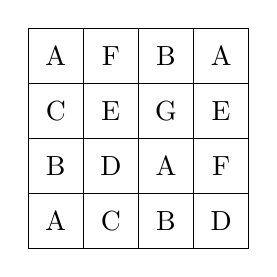
\begin{tikzpicture}[scale=0.7]
\node at (0.5,0.5) {A};
\node at (0.5,1.5) {B};
\node at (0.5,2.5) {C};
\node at (0.5,3.5) {A};
\node at (1.5,0.5) {C};
\node at (1.5,1.5) {D};
\node at (1.5,2.5) {E};
\node at (1.5,3.5) {F};
\node at (2.5,0.5) {B};
\node at (2.5,1.5) {A};
\node at (2.5,2.5) {G};
\node at (2.5,3.5) {B};
\node at (3.5,0.5) {D};
\node at (3.5,1.5) {F};
\node at (3.5,2.5) {E};
\node at (3.5,3.5) {A};
\draw (0,0) grid (4,4);
\end{tikzpicture}
\end{center}
この場合、2つの'E'文字の間の距離は2です。

各文字を別々に考えることで問題を解くことができます。
こう考えると固定文字cを持つ2つのセル間の最小距離を計 算することである。このために、2つのアルゴリズムを考えます。

\emph{アルゴリズム1:}文字cを持つ全てのセルのペアを調べておき、そのセル間の最小距離を計算する。
これには$O(k^2)$の時間がかかる。ここで、$k$は文字$c$を持つセルの数。

\emph{アルゴリズム2:}文字cを持つ各セルから同時に開始する幅優先探索。
文字$c$を持つ2つのセル間の最小距離は$O(n)$で実行できる。

どちらかのアルゴリズムだけをすべての文字に対してそれを使用することでこの問題は解けます。

まず、アルゴリズム1を使用する場合、すべてのセルに同じ文字が含まれる可能性があるため、実行時間
は$O(n^2)$となります。($k=n$となるためです)

アルゴリズム2を使用する場合 、すべてのセルに異なる$n$文字が含まれる可能性があるのでそれぞれに対して
$O(n)$でクエリするため実行時間は $O(n^2)$ となります。

しかし、2つのアルゴリズムを組み合わせて、各文字がグリッドに何回現れるかを事前に計算し、文字ごとにアルゴリズムを使い分けることができます。
ある文字$c$が$k$回出現すると仮定しましょう。$k \le \sqrt n$ならアルゴリズム1を、$k > \sqrt n$ならアルゴリズム2を使いまず。
こうすることで、アルゴリズムの総実行時間は$O(n \sqrt n)$ですむことがわかります。これをもう少し見ていきます。

まず、文字$c$に対してアルゴリズム1を使うとします。
$\sqrt n$回以下出現する文字 $c$のセルと他のセルを比較します。この回数は最大で$O(n \sqrt n)$回です。
したがって、このようなすべてのセルの処理に使われる時間は$O(n \sqrt n)$です。

次に、文字$c$に対してアルゴリズム2を使用することを考えます。このような文字は最大で$\sqrt n$個なので、
それらの文字の処理には$O(n \sqrt n)$個の時間がかかります。

\subsubsection{Batch processing}


次の問題も、$n$個のセルを含む2次元のグリッドを扱います。
初期状態ではまず、1つを除くセルは白です。これに$n - 1$回の操作を行います。
操作は、まず与えられた白いセルから黒いセルまでの最小距離を計算し、次にその白いセルを黒にします。

例を示します。

\begin{center}
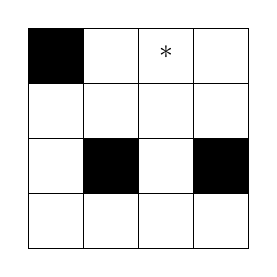
\begin{tikzpicture}[scale=0.7]
\fill[color=black] (1,1) rectangle (2,2);
\fill[color=black] (3,1) rectangle (4,2);
\fill[color=black] (0,3) rectangle (1,4);
\node at (2.5,3.5) {*};
\draw (0,0) grid (4,4);
\end{tikzpicture}
\end{center}

この場面で * のついた白いセルから黒いセルまでの最小距離を計算するしたいとします。
2つ左に移動すれば黒に移動できるので、最小距離は2です。そして、白いセルを黒く塗ります。

\begin{center}
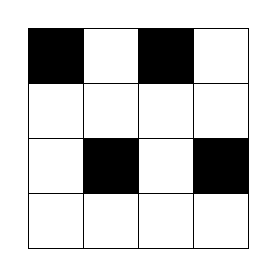
\begin{tikzpicture}[scale=0.7]
\fill[color=black] (1,1) rectangle (2,2);
\fill[color=black] (3,1) rectangle (4,2);
\fill[color=black] (0,3) rectangle (1,4);
\fill[color=black] (2,3) rectangle (3,4);
\draw (0,0) grid (4,4);
\end{tikzpicture}
\end{center}

ここでも2つのアルゴリズムを考えましょう。

\emph{アルゴリズム1:}幅優先探索を用いて、各白セルについて、最も近い黒セルまでの距離を計算する。
これには$O(n)$の時間がかかり、探索後は任意の白セルから黒セルまでの最小距離をO(1)の時間で求められる。

\emph{アルゴリズム2:}黒く塗られたセルのリストを保持しておき、
操作のたびにこのリストをクエリして、また、リストに新しいセルを追加していく。
操作には$O(k)$かかります($k$はリストの長さ)。

上記のアルゴリズムを組み合わせて、演算を$O(\sqrt n)$のバッチに分割します。
各バッチは$O(\sqrt n)$個の操作で構成されます。
各バッチの始めに、アルゴリズム1を実行します。その後、アルゴリズム2を用いて、バッチ内の演算を処理します。
バッチとバッチの間は、アルゴリズム2のリストをクリアします。
各バッチでの演算で、黒セルまでの最小距離は、アルゴリズム1で計算された距離か、 アルゴリズム2で計算された距離のどちらかになります。

その結果、アルゴリズムは$O(n \sqrt n)$ 時間で動作します。
まず、アルゴリズム 1は$O(\sqrt n)$回実行され、各検索は$O(n)$時間です。
次に、バッチで Algorithm 2を使う場合、リストには$O(\sqrt n)$個のセルが含まれ(バッチの間に リストをクリアするため)、
各操作には$O(\sqrt n)$個の時間がかかる。


\section{整数のパーティション - Integer partitions}

平方根アルゴリズムは次の考察に基づき使われることも多くあります。
正の整数$n$を正整数の和で表現した場合、その和は常に最大$O(\sqrt n)$個の異なる数を含む。という事実である。
さて、最大数の異なる数を含む和を構成するためには、小さな数から選んでいく。
今、$1,2,\ldots,k$という数を選ぶと、得られる総和は
\[\frac{k(k+1)}{2}.\]
になる。従って、数の最大量は$k = O(\sqrt n)$となります。
次に、この観測を利用して効率的に解くことができる2つの問題を見ていきましょう。

\subsubsection{ナップザック問題 - Knapsack}

重さの和が$n$である整数の重さのリストが与えられたとしましょう。
我々のタスクは、重みの部分集合を使って作れるすべての重さの数を見つけることである。
例えば、入力が${1, 3, 3}$の場合、可能な和は以下の通りになります。

\begin{itemize}[noitemsep]
\item $0$ (何も選ばない)
\item $1$
\item $3$
\item $1+3=4$
\item $3+3=6$
\item $1+3+3=7$
\end{itemize}

標準的なナップザック問題として捉えると(7.4章参照)、この問題は次のように解けます。
最初の$k$個の重みを用いて和$x$を形成できる場合に1、それ以外は0である関数
$\texttt{possible}(x,k)$を考えます。
重さの和が$n$であることから,重みは最大$n$であるため、
関数のすべての値は動的計画法を用いて$O(n^2)$で計算することができます。

しかし、最大で$O(\sqrt n)$個の\emph{異なる}重りが存在することを利用して、
アルゴリズムをより効率的にすることができます。
まず、重りを同じお守りで構成されるグループに分けて処理します。
各グループを$O(n)$時間で処理す ることができ、$O(n \sqrt n)$とすることができます。

このアイデアは、
これまでに処理したグループを使って形成できる重みの和を記録した配列を使用します。
配列は$n$個の要素からなり、
和$k$が形成できる場合に1、そうでない場合に0となる配列です。
重りのグループを処理するために、配列を左から右へ走査し、
このグループと前のグループを使って形成できる新しい重みの和を記録します。

\subsubsection{文字列構築 - String construction}

長さ$n$の文字列$s$と全ての長さをたしあわせた長さ$m$の文字列の集合$D$があるとき、
$s$が$D$中の文字列の連結して何通りの組み合わせ方があるかを数える問題を考える。
例えば、$\texttt{s}=\texttt{ABAB}$で
$D=\{\texttt{A},\texttt{B},\texttt{AB}\}$とすると、次の4通りが考えられます。

\begin{itemize}[noitemsep]
\item $\texttt{A}+\texttt{B}+\texttt{A}+\texttt{B}$
\item $\texttt{AB}+\texttt{A}+\texttt{B}$
\item $\texttt{A}+\texttt{B}+\texttt{AB}$
\item $\texttt{AB}+\texttt{AB}$
\end{itemize}

動的計画法を用いてこの問題を解くことができます。
ここで、$\texttt{count}(k)$ を $D$ の文字列を用いて接頭辞 $\texttt{s}[0 \ldots k]$ を構成する方法の数とすると、
$\texttt{count}(n-1)$が
問題の答えとなります。これは、Trie木を用いて$O(n^2)$でこの問題を解くことができる。

しかし、文字列のハッシュ値と、
$D$に含まれる文字列の長さが最大$O(\sqrt m)$個であることを利用すれば、
この問題をより効率的に解決することができる。

まず、$D$に含まれる文字列の全てのハッシュ値を含む集合$H$を構築する。

次に、$\texttt{count}(k)$の値を計算する際に、$D$に長さ$p$の文字列が存在するような$p$の値を全て調べておき、
$\texttt{s}[k-p+1 \ldots k]$のハッシュ値を計算して、それがHに属するかどうか確認する。

文字列の長さは最大でも$O(\sqrt m)$ 個なので、この結果、実行時間が$O(n \sqrt m)$のアルゴリズムとなる。

\section{Moのアルゴリズム - Mo's algorithm}

\index{Mo's algorithm}

\key{Mo's algorithm}\footnote{According to \cite{cod15}}は、
静的な配列の区間クエリに応答し、つまり、配列の値が変化しない問題で使用することができます。
各クエリでは、区間$[a,b]$が与えられ、$a$ と $b$ の間の配列要素に基づく値を計算する必要があるとしましょう。
配列は静的なので、クエリは任意の順序で処理できます。
Moのアルゴリズムは、アルゴリズムが効率的に動作することが保証される特別な順序で、クエリを処理していきます。

このアルゴリズムは配列の有効範囲(active range)を保持しておき、有効範囲の問い合わせの答えはすぐににわかるようになっています。
このアルゴリズムはその有効範囲に基づいて問い合わせを処理し、要素を挿入・削除することで
有効範囲の端点を移動させます。このアルゴリズムの時間計算量は$O(n \sqrt n f(n))$ です。
ここで,配列は$n$個の要素を含み,$n$個の問い合わせがあり,要素の挿入と削除には それぞれ$O(f(n))$ の時間がかかるとしましょう。

Moのアルゴリズムのトリックは、クエリの処理順序です。
配列は$k=O(\sqrt n)$要素のブロックに分割され
クエリ $[l_1,r_1]$は、以下のいずれか の場合にクエリ$[l_2,r_2]$ の前に処理されます。

\begin{itemize}
\item $\lfloor l_1/k \rfloor < \lfloor l_2/k \rfloor$ または
\item $\lfloor l_1/k \rfloor = \lfloor l_2/k \rfloor$ かつ $r_1 < r_2$.
\end{itemize}

このように、左端があるブロックにある全てのクエリは、
右端の順にソートされて次々と処理されます。
この順序を用いると、
TODOここ文章直す
左端は$O(\sqrt n)$ステップで$O(n)$ 移 動し、
右端は$O(n)$ステップで$O(\sqrt n)$ 移動し、
アルゴリズム全体は$O(n \sqrt n)$の演算しか実行しないことになります。
このように、両端点はアルゴリズム中に合計$O(n \sqrt n)$ステップ移動することになります。

\subsubsection*{例}

配列の範囲に対応するクエリの集合が与えられて、範囲内の異なる要素の数を数えるクエリに答える問題を考えて見ます。
Moアルゴリズムでは、クエリーは常に同じ方法でソートされますが、
クエリの答えがどのようにストアされるのかはは問題に依存します。
この問題では、$\texttt{count}[x]$は要素xがアクティブ範囲に出現する回数を示す配列\texttt{count}を保持します。
あるクエリから別のクエリに移動すると、アクティブな範囲は変更されます。
例えば、現在の区間が

\begin{center}
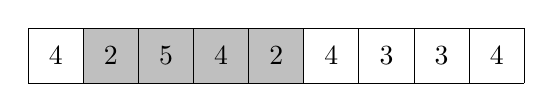
\begin{tikzpicture}[scale=0.7]
\fill[color=lightgray] (1,0) rectangle (5,1);
\draw (0,0) grid (9,1);
\node at (0.5, 0.5) {4};
\node at (1.5, 0.5) {2};
\node at (2.5, 0.5) {5};
\node at (3.5, 0.5) {4};
\node at (4.5, 0.5) {2};
\node at (5.5, 0.5) {4};
\node at (6.5, 0.5) {3};
\node at (7.5, 0.5) {3};
\node at (8.5, 0.5) {4};
\end{tikzpicture}
\end{center}
で、次の区間が次の通りだったとします。
\begin{center}
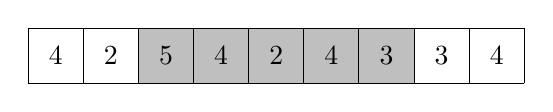
\begin{tikzpicture}[scale=0.7]
\fill[color=lightgray] (2,0) rectangle (7,1);
\draw (0,0) grid (9,1);
\node at (0.5, 0.5) {4};
\node at (1.5, 0.5) {2};
\node at (2.5, 0.5) {5};
\node at (3.5, 0.5) {4};
\node at (4.5, 0.5) {2};
\node at (5.5, 0.5) {4};
\node at (6.5, 0.5) {3};
\node at (7.5, 0.5) {3};
\node at (8.5, 0.5) {4};
\end{tikzpicture}
\end{center}
左の端点が右に1ステップ、右の端点が右に2ステップ移動することになりますね。
各ステップの後、配列\texttt{count}を更新する必要があります。
この更新で$\texttt{count}[x]=1$ になった場合、 クエリに対する答えは1増やし、
$\texttt{count}[x]=0$ になった場合、 クエリに対する答えも 1 つ減らします。
この問題では、各ステップの実行に必要な時間はO(1)であるから、アルゴリ ズムの総時間複雑度は$O(n \sqrt n)$です。
